\chapter{\uppercase{Research Directions} \label{chapter:05}}

Summary of NSF project, some OED stuff perhaps, functional assimilation.

\section{Alternative Experimental Designs}

In this section we return to the nonlinear examples presented in the previous chapter and address the choices made in experimental design.
We demonstrate that the decisions made regarding measurement equipment and/or location have an impact on the reduction of uncertainty and accuracy of the MUD point.

\section{Sequential Inversion}\label{sec:ch05-sequential}

The DCI framework relies on evaluating the ration function $r(\param)$ in $\dimD$--dimensional QoI space, so we turn our attention to addressing the challenges associated with the growth of this space.
As $\dimD$ increases, we must approximate a push-forward distribution with perhaps a fixed number of samples (from model evaluations) $\nsamps$, which represents a considerable source of error since the convergence rate for kernel density estimation with Gaussian kernels is $\mathcal{O} (N^{2+\dimD})$.

For example, suppose we have a time-dependent problem for which hundreds of spatial sensors are providing streams of data.
Approximating a hundred-dimensional space with $\nsamps = 1E3$ or $1E4$ samples (as we have been using for demonstrations), is wrought with problems.
However, either of these values for $\nsamps$ would be sufficient to estimate a one-dimensional distribution.
In some sense, approximating a QoI at each location over time is reasonable, but doing so for all of them simultaneously is not.
To this end, we propose to investigate an approach to solving the parameter estimation problem by performing inversion through a sequence of scalar-valued QoIs rather than employ a vector-valued approach.

We could choose any dimension below $\dimD$, but this sequential-scalar-valued approach provides a starting place and admits a simplicity in exposition.
By choosing a dimension of 1, we can focus solely on the order in which QoIs are inverted and dismiss the additional complexity of enumerating the combinations of QoI when dimensions can vary.
We also choose to use a linear map for convenience so that we can use the analytical solutions presented in the previous chapter without concern for approximation error.

With each iteration in the sequence of inverse problems, we are in-effect trying to explain measurements that constitute a single QoI at the expense of accuracy in others.
By contrast, the vector-valued approach seeks accuracy in all of the simultaneously.
This trade off is all about convenience, since 1-dimensional problems are computationally ``cheap,'' we can iterate through many more of them for the same computational cost.
Since by the time we finish iterating through all available QoI, the error in $Q^{(1)}$ may have been allowed to drift quite significantly away from its solution contour through the sequence of inverting through $Q^{(1)}, Q^{(2)}, \dots Q^{(100)}$.
To address this, we perform multiple passes through our set of QoI.
Borrowing from other sequential algorithms, these ``epochs'' will allow us to iterate until the solution stops changing by some predefined relative threshold, representing a lack of ``learning'' through continued effort.

We study the following motivating two-dimensional example with QoI defined by ten equispaced rotations of the unit vector $[0, 1]$ through the first two Euclidean quadrants.
We first plot the result of a single epoch in Fig.~\ref{fig:iterative-linear-demo}
\begin{figure}
  \centering
  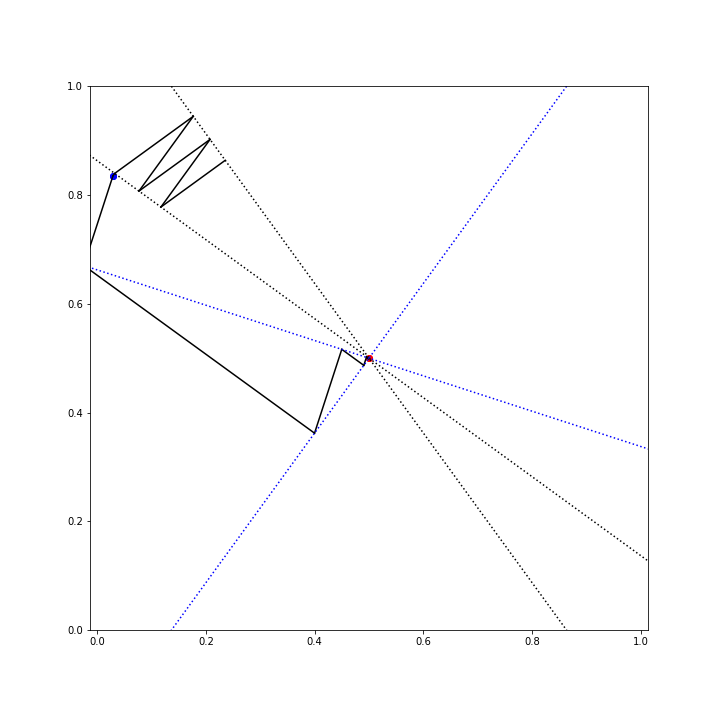
\includegraphics[width=0.475\linewidth]{examples/iterative/10D-firstepoch}
  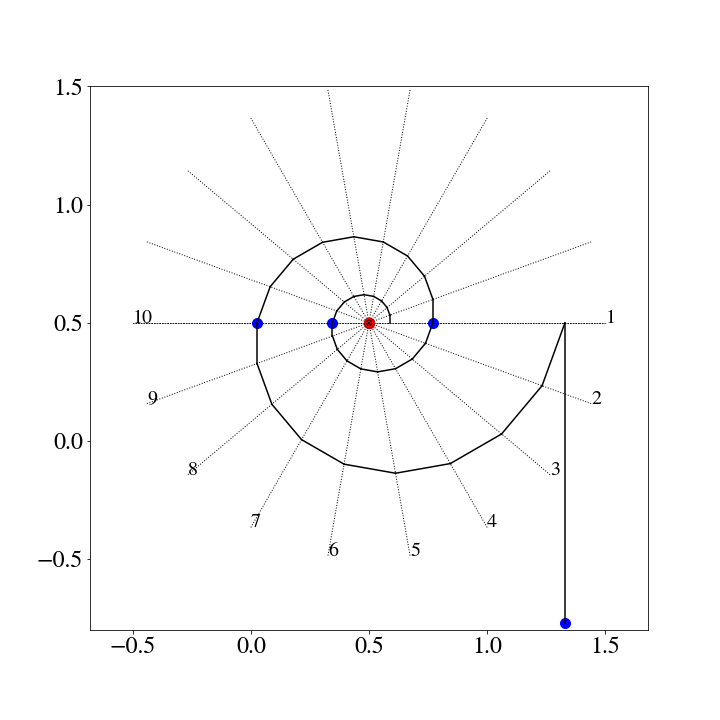
\includegraphics[width=0.475\linewidth]{examples/iterative/10D-fewepochs}

  \caption{
  Dotted lines show the solution contours for each row of the operator $A$.
  (Left): First epoch for iterating through 10 QoI.
  (Right): Three more epochs allows our estimate to get much closer to the true value.
  }
  \label{fig:iterative-linear-demo}
\end{figure}

The spiral shape is a result of the underlying geometry of this QoI map defined by rotations. The successive rows are so similar to each other that very little is ``learned'' between each iteration; the projection doesn't cover a large distance in $\pspace$.
To drive this point home, we choose two pairs of indices from among the ten available in order to define two QoI maps, the contours for which we plot in different colors in Fig.~\ref{fig:iterative-linear-demo-pair}.
We solve a total of ten 1-D inverse problems for each of them (five epochs) to match the budget of the previous example (with ten maps and one epoch).

\begin{figure}
  \centering
  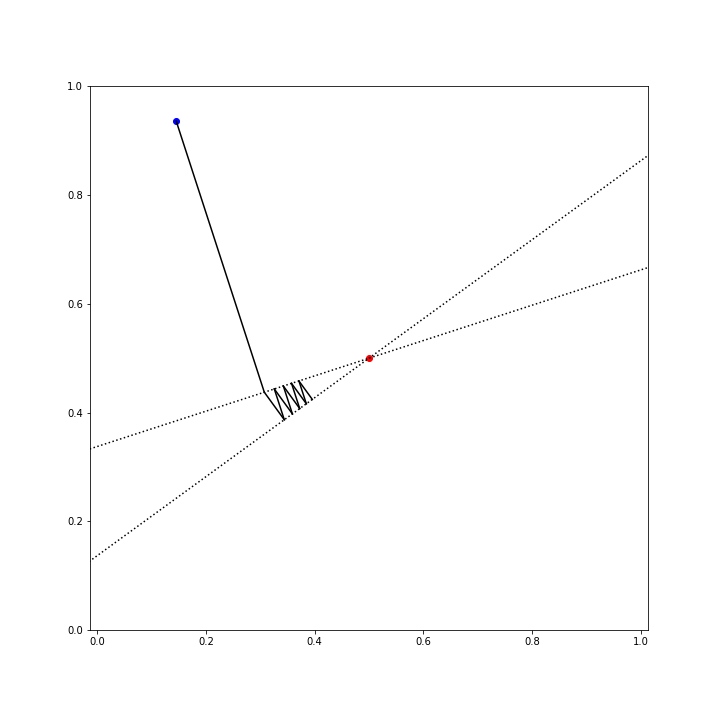
\includegraphics[width=0.475\linewidth]{examples/iterative/10D-fewepochs-pair}
  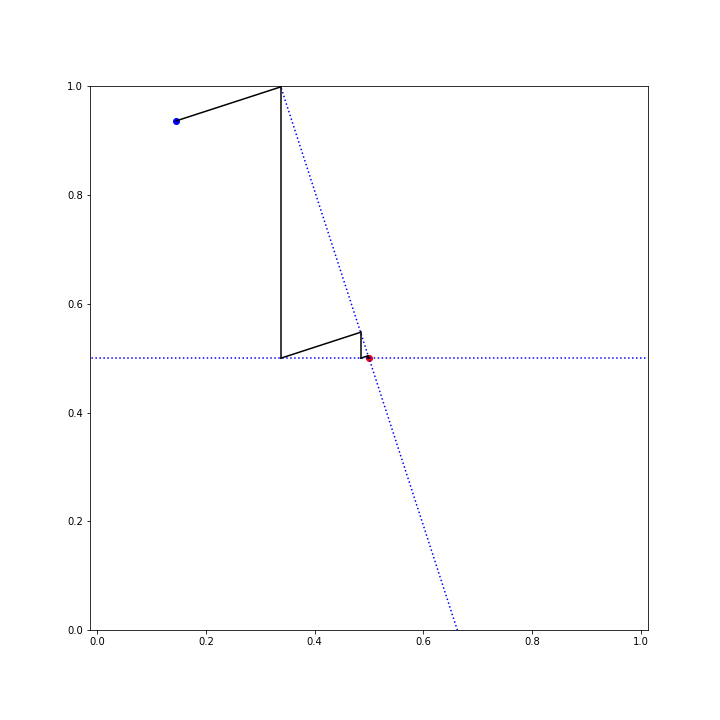
\includegraphics[width=0.475\linewidth]{examples/iterative/10D-fewepochs-pair-alt}
  \caption{
  Iterating through five epochs of two QoI, each formed by picking two of the ten available rows of $A$ at random.
  }
  \label{fig:iterative-linear-demo-pair}
\end{figure}

We observe that in Fig~\ref{fig:iterative-linear-demo-pair}, we are able to achieve much greater accuracy in estimating the true parameter value than in the case of Fig~\ref{fig:iterative-linear-demo}.
The reason for this difference is that there is more mutually distinct information between successive iterations of a pair of random rows of $A$ than there is between adjacent rows, as measured by the angle between the solution contours.
Had we chosen a pair of rows that were orthogonal, the initial mean would converge to the reference value in a single epoch (two iterations), since there is no redundancy in information whatsoever.
We show this in the left half of Figure~\ref{fig:iterative-linear-demo-smart} for two orthogonal pairs.
If we instead choose to perform no a-priori analysis of the rows of $A$ and iterated through them at random, we actually also manage to accomplish a lot more accuracy for the same amount of iterations, as seen in the right half of the figure.

\begin{figure}
  \centering
  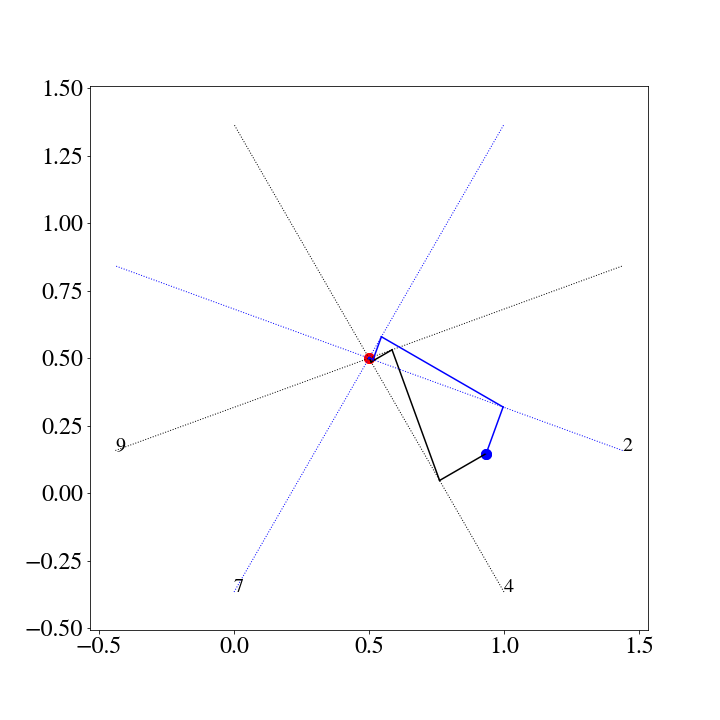
\includegraphics[width=0.475\linewidth]{examples/iterative/10D-firstepoch-pair-smart}
  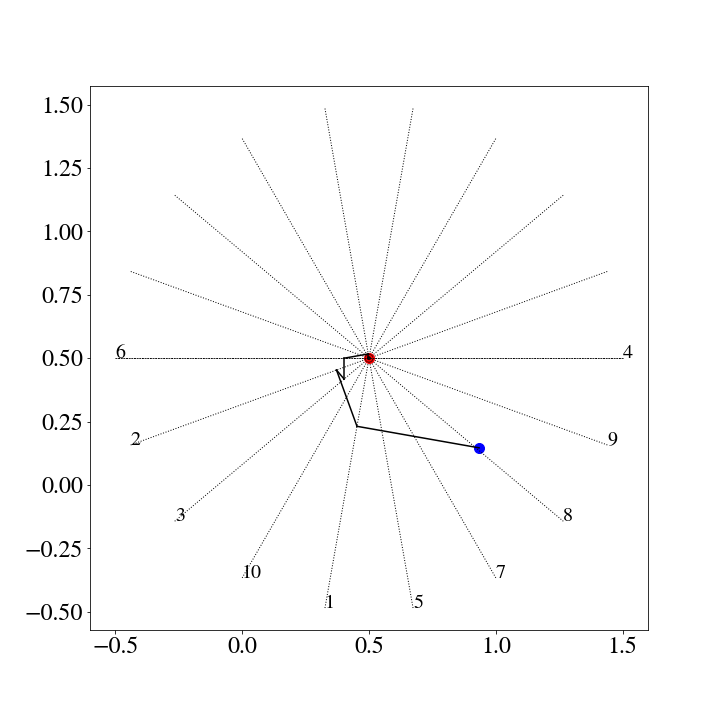
\includegraphics[width=0.475\linewidth]{examples/iterative/10D-firstepoch-rand}
  \caption{
  If we are careful with how we construct our maps or choose our iteration strategy, we can achieve considerably more accurate solutions with the same computational cost.
  (Left): Iterating through a single epoch with a QoI formed by picking rows of $A$ which exhibit mutual orthogonality.
  (Right): Iterating through the rows of $A$ at a random order for a single epoch results in considerably more accuracy than doing so in the original order of rows of $A$.
  }
  \label{fig:iterative-linear-demo-smart}
\end{figure}

To make these results more concrete, we propose the following example:
We limit ourselves to solving 100 inverse problems (i.e. up to ten epochs for this map), with the \emph{only} difference between approaches being the order in which the rows of $A$ are used.
First, we use the QoI as they are presented to us, in order with respect to increased rotation angle (which defines the rows of $A$).
Next, we shuffle the rows and then perform ten epochs.
Lastly, we create an ordering based on a random shuffling of the indices representing the rows of $A$, repeated ten times, for which only a single epoch is performed.
The latter approach is similar to the second in that the same problems are solved the same number of times overall, but it lifts the restriction that a row must only be used once in each effective ``epoch''.

\begin{figure}
  \centering
  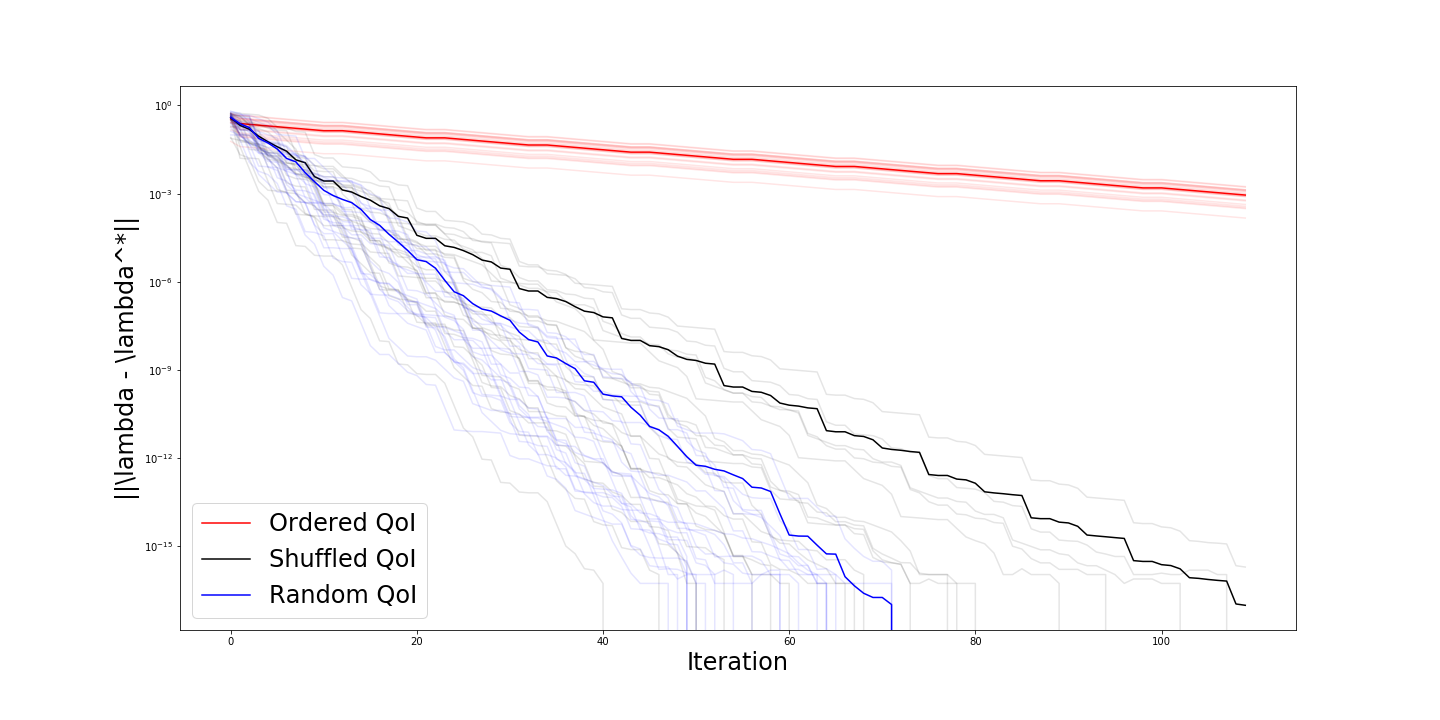
\includegraphics[width=0.95\linewidth]{examples/iterative/10D-convergence-comparison}
  \caption{
  Twenty different initial means are chosen and iterated on for three approaches.
  Individual experiments are transparent and the mean error is shown as solid lines.
  In the \emph{Ordered} approach, we iterate through the rows of $A$ as they are given to us for ten epochs.
  \emph{Shuffled QoI} refers to establishing a different random ordering of the rows of $A$ for each trial, and then
  using this ordering for ten epochs.
  Finally, in the \emph{Random QoI} approach, we choose a QoI at random for each of 100 iterations, where the ordering still ensures each row gets used ten times, representing the same overall set of inverse problems solved as the other two.
  }
  \label{fig:iterative-convergence-comparison}
\end{figure}

We see in Figure~\ref{fig:iterative-convergence-comparison} that using the rows of $A$ sequentially performs very poor, which aligns with ``spiraling'' seen in Figure~\ref{fig:iterative-linear-demo} where the first few epochs were plotted.
Shuffling the rows but requiring that every tenth iteration to use the same row (i.e., ensure same ordering for each epoch), leads to a considerable improvement by which sixteen decimal places of accuracy are achieved in under $100$ iterations.
In a few instances, the shuffled approach stumbles on an ordering that accelerates convergence, likely due to orthogonal pairs of rows in the shuffled order.
These cases exhibit the kind of behavior we saw in the left panel of Fig~\ref{fig:iterative-linear-demo-smart}; in other words, sometimes our random shuffling finds the ``smart'' rows to iterate through.
Since the ordering has no dependence on iteration number in the approach where we use random rows, we have more opportunities to find these successive orthogonal pairings, and so we see that on average, it takes fewer iterations to achieve the same accuracy.



\section{Addressing Model Assumptions}\label{sec:ch05-variance}

What if we don't know the variance? How does mis-estimating it affect our solutions?

Multiplicative noise - handled in a straightforward way, maybe put an example here and leave it at that? Put it in appendix?


\section{Leveraging Data in Different Ways}\label{sec:ch05-data}

This section is effectively addressing how to use more data in different ways.

Would be nice to see a data-driven map done with the set-based framework first as an example.
May be appropriate in example for Ch 4.

\section{Optimal Experimental Design}\label{sec:ch05-oed}

Algorithm for sequentially choosing QoI, brief discussion of trade-offs of accuracy/precision.

\section{Machine-Learning Enhancements}\label{sec:ch05-ml}

how can we automate this process? Some mixture of sequential (how can we incorporate a new data point? start over? re-solve the problem? what's the cost?) approximations, maybe switching between the two approaches (set-based to reduce the parameter space, use that as the new initial).
